\section{Expected Event Rate and Oscillation Parameters}
%{\it Assigned to:} {\bf Mayly Sanchez} 
\label{sec:physics-lbnosc-osc}




The signal for \nue (\anue) appearance is an excess of \dword{cc} %charged-current (CC) 
\nue and \anue interactions over the expected background in the far detector.  The background to \nue appearance is composed of: (1) \dword{cc} interactions of \nue and \anue intrinsic to the beam; (2) misidentified \dword{nc} %neutral current (NC) 
interactions;  (3) misidentified \numu and \anumu \dword{cc} interactions; and (4) $\nu_\tau$ and $\bar{\nu}_\tau$ \dword{cc} interactions in which the $\tau$s decay leptonically into electrons/positrons. \dword{nc} and $\nu_\tau$ backgrounds emanate from interactions of higher-energy neutrinos that feed down to lower reconstructed neutrino energies due to missing energy in unreconstructed final-state neutrinos. The selected NC and \dword{cc} \numu generally include an asymmetric decay of a relatively high energy $\pi^0$ coupled with a prompt photon conversion.

A full simulation chain that includes the beam flux, the \dword{genie} %GENIE 
neutrino interaction
generator~\cite{Andreopoulos:2009rq}, and \dword{geant4}-based %Geant4-based 
detector models has been implemented. Section~\ref{sec:physics-lbnosc-flux} describes the beam design, simulated flux, and associated uncertainties.
Event rates are based on a 1.2~MW neutrino beam and corresponding protons-on-target per year assumed to be 1.1 $\times 10^{21}$ POT.  These numbers assume a combined uptime and efficiency of the \dword{fnal} accelerator complex and the \dword{lbnf} beamline of 56\%.
An upgrade to 2.4 MW is assumed after six years of data collection. The neutrino interaction model has been generated using \dword{genie} 2.12 and the choices of models and tunes as well as associated uncertainties are described in detail in Section~\ref{sec:nu-osc-05}. The performance parameters for the near and far detectors are described in detail in Sections~\ref{sec:physics-lbnosc-ND} and~\ref{sec:physics-lbnosc-FD}. 
 Near Detector Monte Carlo has been generated using \dword{geant4} and a parameterized reconstruction based on true energy deposits in the active detector volumes has been used as described in Section~\ref{sec:physics-lbnosc-ND}.
 Far detector Monte Carlo has been generated using LArSoft and the reconstruction and event selection in the Far Detector has been fully implemented, as described in Section~\ref{sec:physics-lbnosc-FD}. Uncertainties associated with detector effects in the near and far detectors are described in Section~\ref{sec:physics-lbnosc-syst}. The methods used in calculating the DUNE sensitivity results are described in Section~\ref{sec:physics-lbnosc-sens} and these results based on the full framework are shown in Section~\ref{sec:physics-lbnosc-results}.

The neutrino oscillation parameters and the uncertainty on those parameters are taken from the \dword{nufit}~\cite{Esteban:2018azc,nufitweb} global fit to neutrino data; the
values are given in Table~\ref{tab:oscpar_nufit}.  (See also
\cite{deSalas:2017kay} and \cite{Capozzi:2017yic} for other recent global fits.) The sensitivities in this chapter are shown assuming normal ordering; this is an arbitrary choice for simplicity of presentation.

Event rates are presented as a function of calendar years and are calculated with the following assumed deployment plan, which is based on a technically limited schedule.
\begin{itemize}
    \item Start of beam run: Two \dword{fd} module %FD 
    volumes for total fiducial mass of 20 kt, 1.2 MW beam
    \item After one year: Add one \dword{fd} module  volume for total fiducial mass of 30 kt
    \item After three years: Add one \dword{fd} module  volume for total fiducial mass of \fdfiducialmass
    \item After six years: Upgrade to 2.4 MW beam
\end{itemize}

\begin{table}[]
    \centering
    \begin{tabular}{lcc}
 Parameter &    Central Value & Relative Uncertainty \\
\toprowrule
$\theta_{12}$ & 0.5903 & 2.3\% \\ \colhline
$\theta_{23}$ (NO) & 0.866  & 4.1\% \\ 
$\theta_{23}$ (IO) & 0.869  & 4.0\% \\ \colhline
$\theta_{13}$ (NO) & 0.150  & 1.5\% \\ 
$\theta_{13}$ (IO) & 0.151  & 1.5\% \\ \colhline
$\Delta m^2_{21}$ & 7.39$\times10^{-5}$~eV$^2$ & 2.8\% \\ \colhline
$\Delta m^2_{32}$ (NO) & 2.451$\times10^{-3}$~eV$^2$ &  1.3\% \\
$\Delta m^2_{32}$ (IO) & -2.512$\times10^{-3}$~eV$^2$ &  1.3\% \\
    \end{tabular}
    \caption[Parameter values and uncertainties from a global fit to neutrino oscillation data]{Central value and relative uncertainty of neutrino oscillation parameters from a global fit~\cite{Esteban:2018azc,nufitweb} to neutrino oscillation data. Because the probability distributions are somewhat non-Gaussian (particularly for $\theta_{23}$), the relative uncertainty is computed using 1/6 of the 3$\sigma$ allowed range from the fit, rather than the 1$\sigma$ range.   For $\theta_{23}$, $\theta_{13}$, and $\Delta m^2_{31}$, the best-fit values and uncertainties depend on whether normal mass ordering (NO) or inverted mass ordering (IO) is assumed.}
    \label{tab:oscpar_nufit}
\end{table}
%\end{cdrtable}

Figures~\ref{fig:appspectra} and~\ref{fig:disspectra} show the expected rate of selected events for \nue appearance and \numu disappearance, respectively, including expected flux, cross section, and oscillation probabilities, as a function of reconstructed neutrino energy at a baseline of
\SI{1300}{\km}. The spectra are shown for a \num{3.5}~year (staged) exposure each for neutrino and antineutrino beam mode, for a total run time of seven %\num{7}
years. Tables~\ref{tab:apprates} and~\ref{tab:disrates} give the integrated rate for the \nue %$\nu_e$ (see defs.tex}
appearance and \numu %$\nu_\mu$ 
disappearance spectra, respectively.  

\begin{dunefigure}[\nue and \anue appearance spectra]{fig:appspectra}
{\nue and \anue appearance spectra: Reconstructed energy distribution of selected \nue \dword{cc}-like events assuming 3.5 years (staged) running in the neutrino-beam mode (left) and antineutrino-beam mode (right), for a total of seven years (staged) exposure.  The plots assume normal mass ordering and include curves for $\mdeltacp = -\pi/2, 0$, and $\pi/2$.}
 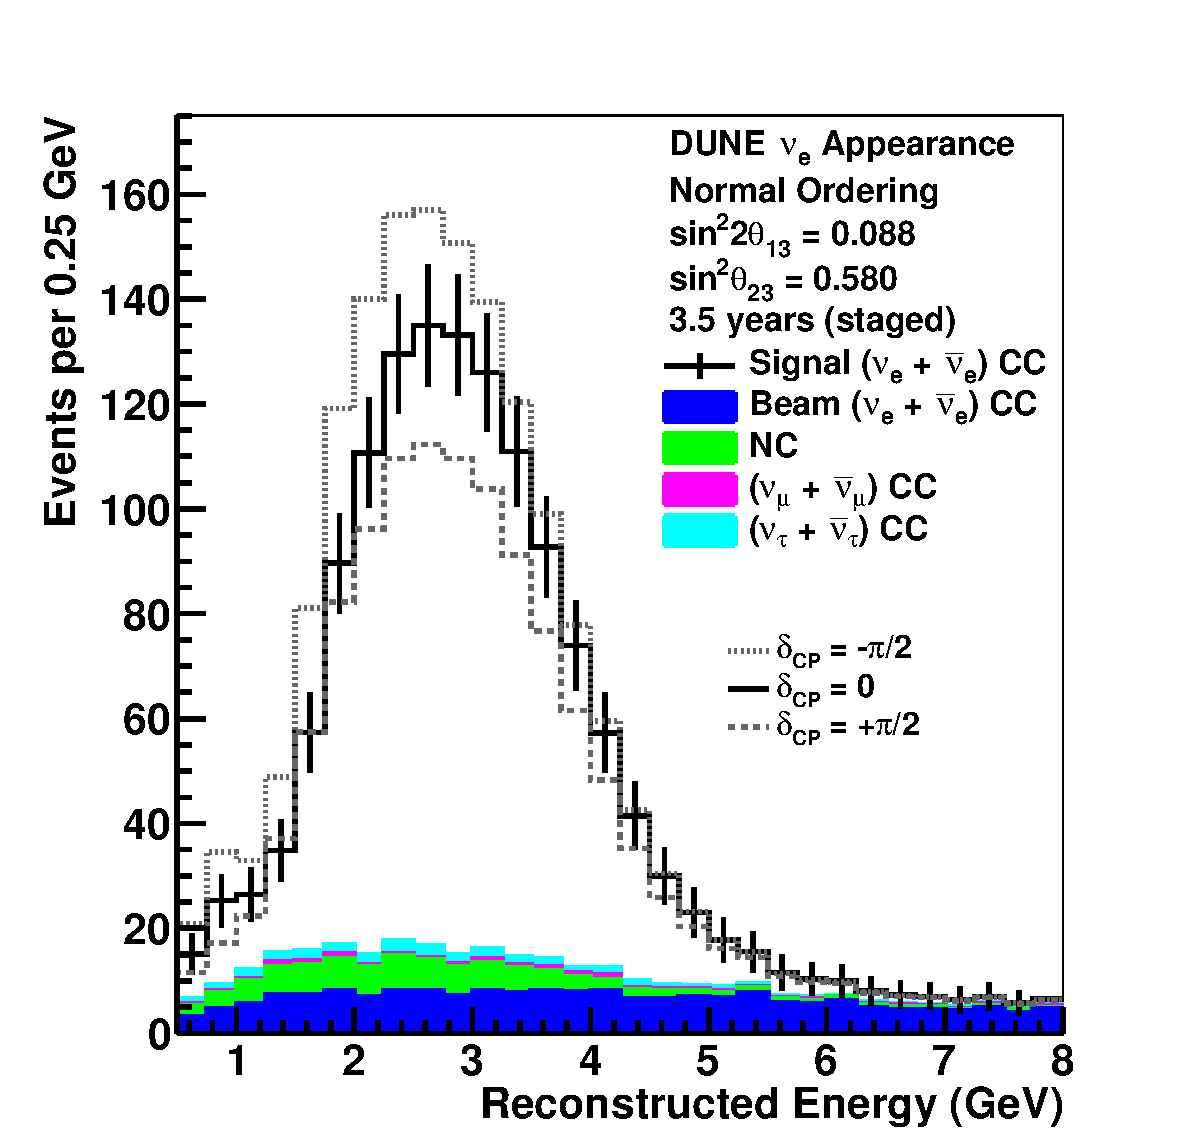
\includegraphics[width=0.49\textwidth]{spec_app_nu_varydcp.pdf}
 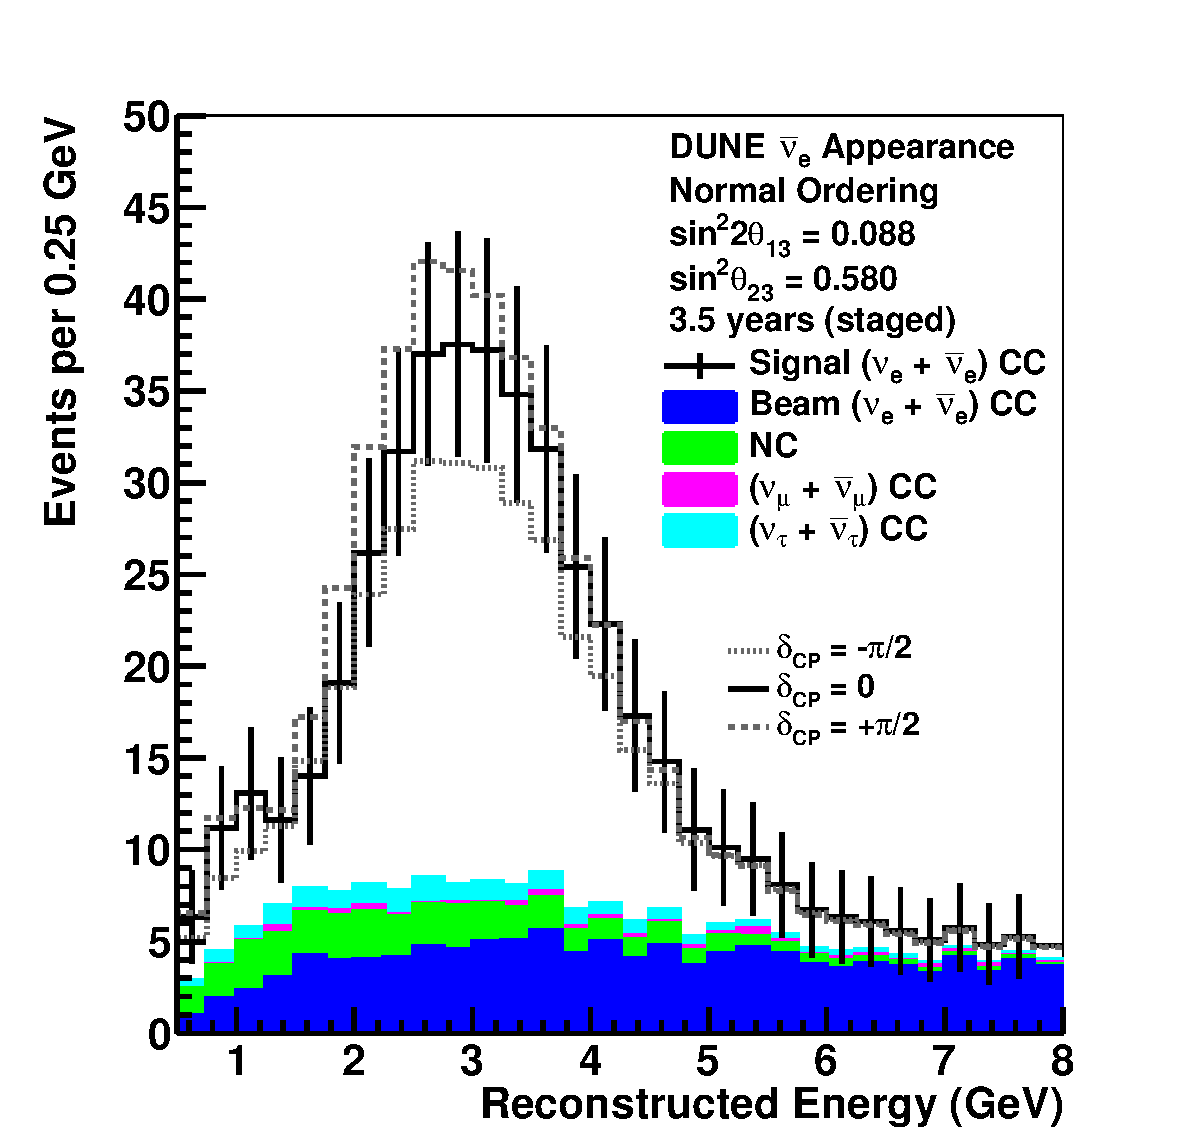
\includegraphics[width=0.49\textwidth]{spec_app_anu_varydcp.pdf}
\end{dunefigure}



\begin{dunefigure}[\numu and \anumu disappearance spectra]{fig:disspectra}
{\numu and \anumu disappearance spectra: Reconstructed energy distribution of selected $\nu_{\mu}$ \dword{cc}-like events assuming 3.5 years (staged) running in the neutrino-beam mode (left) and antineutrino-beam mode (right), for a total of seven years (staged) exposure. The plots assume normal mass ordering.}
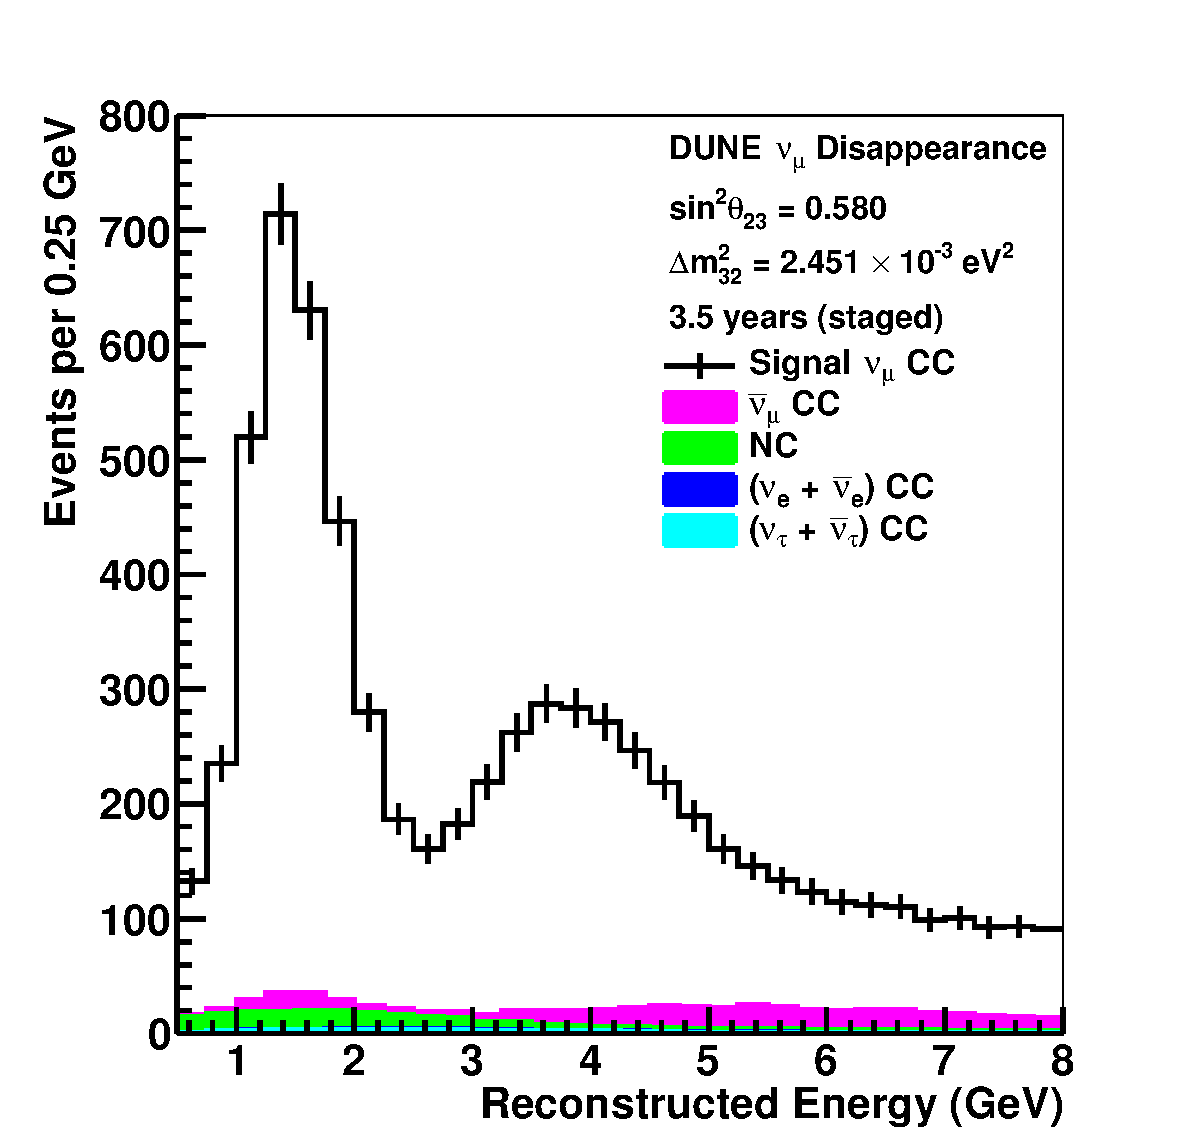
\includegraphics[width=0.49\textwidth]{spec_dis_nu.pdf}
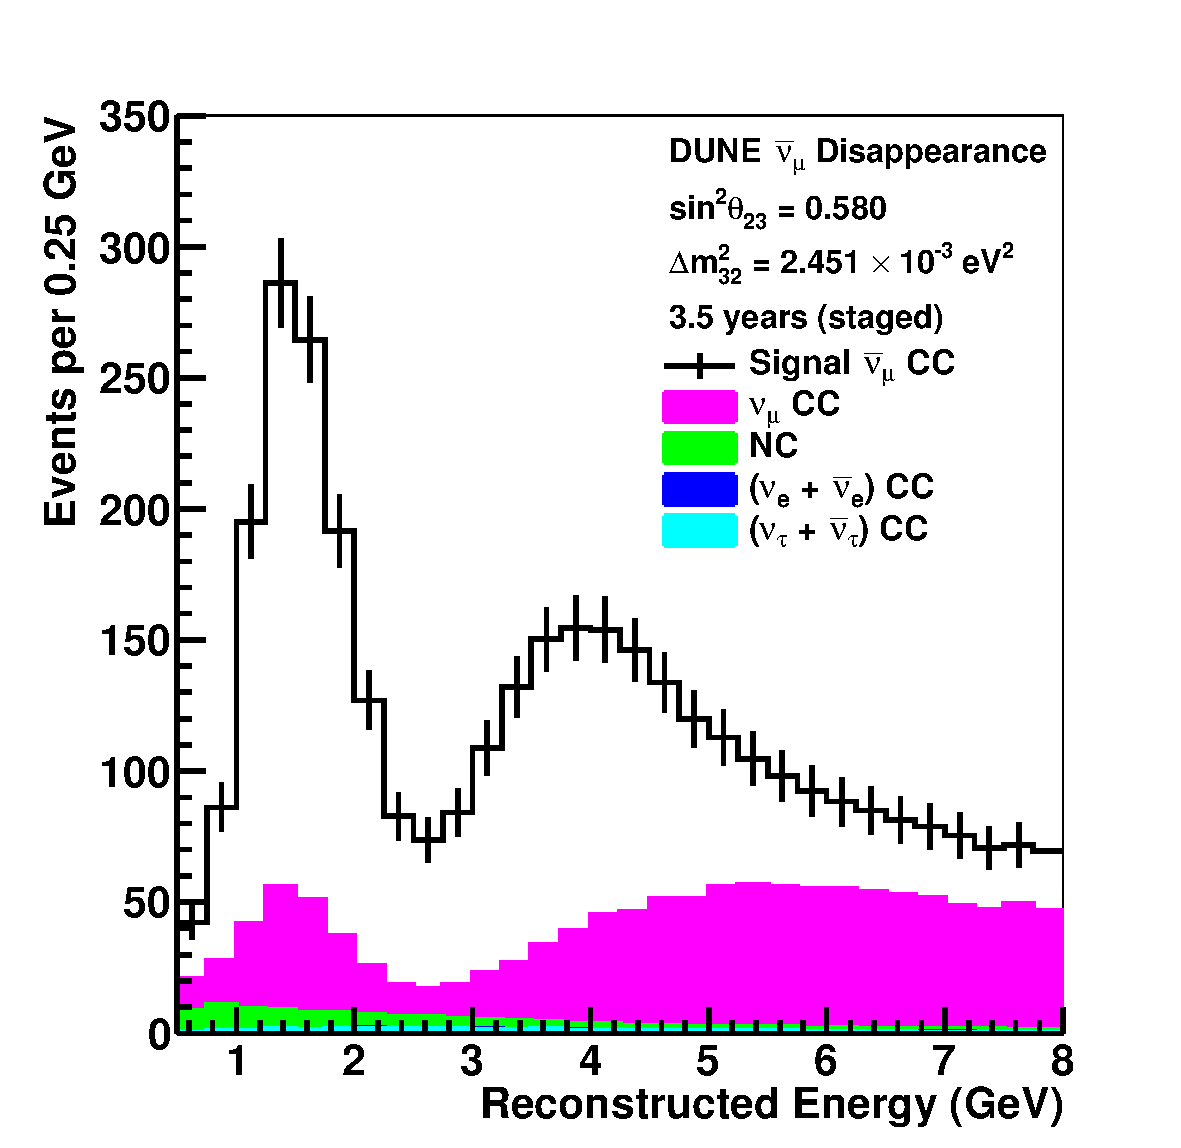
\includegraphics[width=0.49\textwidth]{spec_dis_anu.pdf}
\end{dunefigure}



\begin{dunetable}
[\nue and \anue appearance rates]
{lrr}
{tab:apprates}
{\nue and \anue appearance rates: Integrated rate of selected $\nu_e$ \dword{cc}-like events between 0.5 and 8.0~GeV assuming a \num{3.5}-year (staged) exposure in the neutrino-beam mode and antineutrino-beam mode.  The signal rates are shown for both normal mass ordering (NO) and inverted mass ordering (IO), and all the background rates assume normal mass ordering.  All the rates assume $\mdeltacp = 0$.}
& Expected Events (3.5 years staged) \\ \toprowrule
 $\nu$ mode & \\
 \colhline 
 \nue Signal NO (IO) & 1092 (497) \\
 \anue Signal NO (IO) & 18 (31) \\
  \colhline
 Total Signal NO (IO) & 1110 (528) \\
  \colhline 
 Beam $\nu_{e}+\bar{\nu}_{e}$ \dword{cc} background & 190 \\
 \dword{nc} background & 81 \\
 $\nu_{\tau}+\bar{\nu}_{\tau}$ \dword{cc} background & 32 \\
 $\nu_{\mu}+\bar{\nu}_{\mu}$ \dword{cc} background & 14 \\
  \colhline
 Total background & 317 \\
 \toprowrule
 $\bar{\nu}$ mode & \\
 \colhline 
 \nue Signal NO (IO) & 76 (36) \\
 \anue Signal NO (IO) & 224 (470) \\
  \colhline
 Total Signal NO (IO) & 300 (506) \\
  \colhline 
 Beam $\nu_{e}+\bar{\nu}_{e}$ \dword{cc} background & 117 \\
 \dword{nc} background & 38 \\
 $\nu_{\tau}+\bar{\nu}_{\tau}$ \dword{cc} background & 20 \\
 $\nu_{\mu}+\bar{\nu}_{\mu}$ \dword{cc} background & 5 \\
  \colhline 
 Total background & 180 \\
\end{dunetable}




\begin{dunetable}
[\numu and \anumu disappearance rates]
{lrr}
{tab:disrates}
{\numu and \anumu disappearance rates: Integrated rate of selected $\nu_{\mu}$ \dword{cc}-like events between 0.5 and 8.0~GeV assuming a \num{3.5}-year (staged) exposure in the neutrino-beam mode and antineutrino-beam mode.  The rates are shown for normal mass ordering and $\mdeltacp = 0$.}
& Expected Events (3.5 years staged)\\ \toprowrule
  $\nu$ mode & \\
 \colhline %\toprowrule
 \numu Signal & 6200 \\
 \colhline %\toprowrule
  \anumu \dword{cc} background & 389 \\
 \dword{nc} background & 200 \\
 $\nu_{\tau}+\bar{\nu}_{\tau}$ \dword{cc} background & 46 \\
 $\nu_e+\bar{\nu}_e$ \dword{cc} background & 8 \\
%  \toprowrule
%  Total Background & xxxx \\
 \toprowrule
% \toprowrule
 $\bar{\nu}$ mode  & \\
\colhline % \toprowrule
 \anumu Signal & 2303 \\
\colhline % \toprowrule
  \numu \dword{cc} background & 1129 \\
 \dword{nc} background & 101 \\
 $\nu_{\tau}+\bar{\nu}_{\tau}$ \dword{cc} background & 27 \\
 $\nu_e+\bar{\nu}_e$ \dword{cc} background & 2 \\
\end{dunetable}

